\documentclass[sigconf]{acmart}

\usepackage{graphicx}
\usepackage{hyperref}
\usepackage{todonotes}

\usepackage{endfloat}
\renewcommand{\efloatseparator}{\mbox{}} % no new page between figures

\usepackage{booktabs} % For formal tables

\settopmatter{printacmref=false} % Removes citation information below abstract
\renewcommand\footnotetextcopyrightpermission[1]{} % removes footnote with conference information in first column
\pagestyle{plain} % removes running headers

\newcommand{\TODO}[1]{\todo[inline]{#1}}

\begin{document}
\title{Big Data Analytics in Identifying Factors Affecting Bitcoin}


\author{Ashok Kuppuraj}
\orcid{1234-5678-9012}
\affiliation{%
  \institution{Indiana University}
  \streetaddress{}
  \city{Bloomington} 
  \state{Indiana} 
  \postcode{43017-6221}
}
\email{akuppura@iu.edu}


% The default list of authors is too long for headers}
\renewcommand{\shortauthors}{G. v. Laszewski}


\begin{abstract}
Pricing of Blockchain based cryptocurrencies are like a black box, as per theory the pricing compared to U.S dollar is based on a number of transactions however lot other factors like Dollar price, social media, Online threats supersede the transaction count. Big data and Analytics helps to identify the metrics impacting this variation and identify the correlation between them.
\end{abstract}

\keywords{i523, hid324, Big data, Predictive analytics, Random Forest, correlation, Blockchain, Bitcoin, Ethereum}


\maketitle

\section{Introduction}
The start of the 21st century witnessed the evolution of various disruptive technologies, right from Big data, IoT, VR to Blockchain. When it comes to the blockchain, the sole winner is Bitcoin, with the growth rate of over 1327 percent \cite{coingrowth:online}, Bitcoin is disrupting the way banking system works. As the Bitcoin grows the acceptance and adoption grow along with that. Similar to any other currency in the world, Bitcoin's price deviates widely towards the positive side which created the opportunity for investment in it. Even though the same is not widely accepted everywhere, there is a grace to own Bitcoin citing its growth rate. Though the transaction counts haven't grown up, the retention of the coin has grown up making it a Digital Gold \cite{Retain:online}.


\section{Bitcoin}
Bitcoin is a progressed cryptographic cash and shared ledger that is completely decentralized, which implies it relies upon peer-to-peer trades with no bureaucratic oversight. Trades and liquidity inside the framework are somewhat based on cryptography. The concept was first introduced in 2009  \cite{Bitcoin} and is at this moment a prospering open-source gathering and portion sort out. In perspective of the uniqueness of Bitcoin's tradition and its creating choice, the Bitcoin is grabbing stacks of thought from associations, clients, and monetary experts alike. Specifically, for this technology to thrive, we need to recreate budgetary organizations and things that starting at now exist in our traditional, fiat cash world, make them available and specially fitted to Bitcoin, and other rising computerized types of cash.
In technical terms, Bitcoin's is a shared ledger or a database running by a set of clusters, as the clustering is involved, a competition is set for the individual machines to acquire and update the ledger. The competition is in terms of hashing problem. The hashing needs multiple GPU's to perform validations and update the ledger. This competition eliminates the slower machines to be part of the network and improve the infrastructure's capacity, only by winning the competition a machine can be awarded some Bitcoin as an incentive. Since one machine cannot process the competition problem, a set of peers come together to form a Mining pool and share their capacity and the incentives. We can gather useful mining statistics information from these mining pools.
 
 \section{Price prediction}
 The Bitcoin market's cash-related basic is, clearly, a securities trade. To support money related to reward, the stock market prediction has turned out to be known ground which can be reused with the presence of high-repeat,low-dormancy trading hardware joined with solid machine learning figurings. Henceforth, it looks good that this desire is imitated in the domain of Bitcoin, as the framework expands more conspicuous liquidity and more people develop an excitement for placing profitably in the structure. To do accordingly, it is essential to utilize machine learning and Big data advancements to foresee the cost of Bitcoin \cite{stock}.
 
 
 \subsection{Data Source}
 As Bitcoin is a decentralized and a transparent system, all the source of data can be gathered from the peer-to-peer networks. This peer-to-peer network is called as Bitcoin-mining pool \cite{1:online}.The rate of block creation is adjusted every 2016 blocks to aim for a constant two week adjustment period (equivalent to 6 per hour.) The number of Bitcoins generated per block is set to decrease geometrically, with a 50 reduction every 210,000 blocks, or approximately four years. The result is that the number of bitcoins in existence is not expected to exceed 21 million \cite{2:online}.
The true source of data for Bitcoin analysis would be from Bitcoin mining pool. Coinbase is one of the main members of bitcoin pool from which we can gather mining statistics. In the process of identifying the features impacting Bitcoin's price fluctuations, not only the transaction volume impacts, even the popularity and people's trend towards it impact the price of the coins. Hence, data from Google is also gathered. As a currency's price also been altered by its exchange, supply, and demand, Ethereum's price data and transactional data is also acquired from Ethereum's exchange point.
With all these data sources, we analyze the features impacting the Bitcoin's market price. 
 
 
 \subsection{Feature Selection}
 Feature selection is one of the vital steps in any meaningful analysis of an expected outcome. A set of features have been selected to analyze its interdependence with Bitcoin's evaluation. The features are selected based on three wide areas, the first is Bitcoin mining data, second is social data and the last one is exchange data.
 The internal activities in the Bitcoin's infrastructure definitely reflect the changes or the fluctuations in the Bitcoin's network, Bitcoin's mining data is gathered from Coinbase. This is extracted from the web service API provided by Quandl.com \cite{3:online}. By making a REST call, CSV files containing the historical data is downloaded and processed.
 The second is the social data, which is extracted as a static data from Google trends \cite{google:online}, the main reason behind this data is when the popularity grows people tend to know or show interest in being part of the growth. With the impressive growth of more than 1000 percent in a year, this is considered as an important data.
 The last one is the exchange data, as a currencies price is directly proportional to the supply and demand, the supply of the currency can be impacted by the exchange to other currencies or commodity \cite{4:online}. Ethereum is known to show a similar pattern in terms of growth and deviations \cite{Ethereum:online}. Hence, there's price in US dollars and transaction volume is considered one of the features.

\section{Big data in Feature Analysis and Algorithm's execution}
Feature extraction, transformation, and prediction can be synonymous with a conventional ETL methodology. Though few of the extraction is handled manually and the volume is comparably low, it is assumed that the data volume will be increased by modifying the extraction to real-time systems. When the extraction systems are changed, our code must be able to handle streaming data which can be related to "variety and volume " of the data. The next step is validating the data for anomalies, data miss and cleanse the data of issues which is synonymous with data cleansing. The later one is data processing, which includes data processing with multiple iterations and permutation consuming a lot of memory and other resources. These processing needs lead us in adopting Big data technologies in the entire lifecycle of the implementation.
Apache Spark framework is identified as the end-to-end processing environment which is pre-loaded with redundancy, fault tolerance, in-memory processing, parallel processing, streaming, and Machine learning modules.

\subsection{Execution with Apache Spark}
''Apache Spark is a fast and general-purpose cluster computing system. It provides high-level APIs in Java, Scala, Python and R, and an optimized engine that supports general execution graphs''. It also provides extensive support to Machine learning libraries(MLlib) and to streaming through Spark Streaming. The in-memory processing is implemented with the help of Resilient distributed dataset (RDD) \cite{5:online}.

\begin{figure}[!ht]
  \centering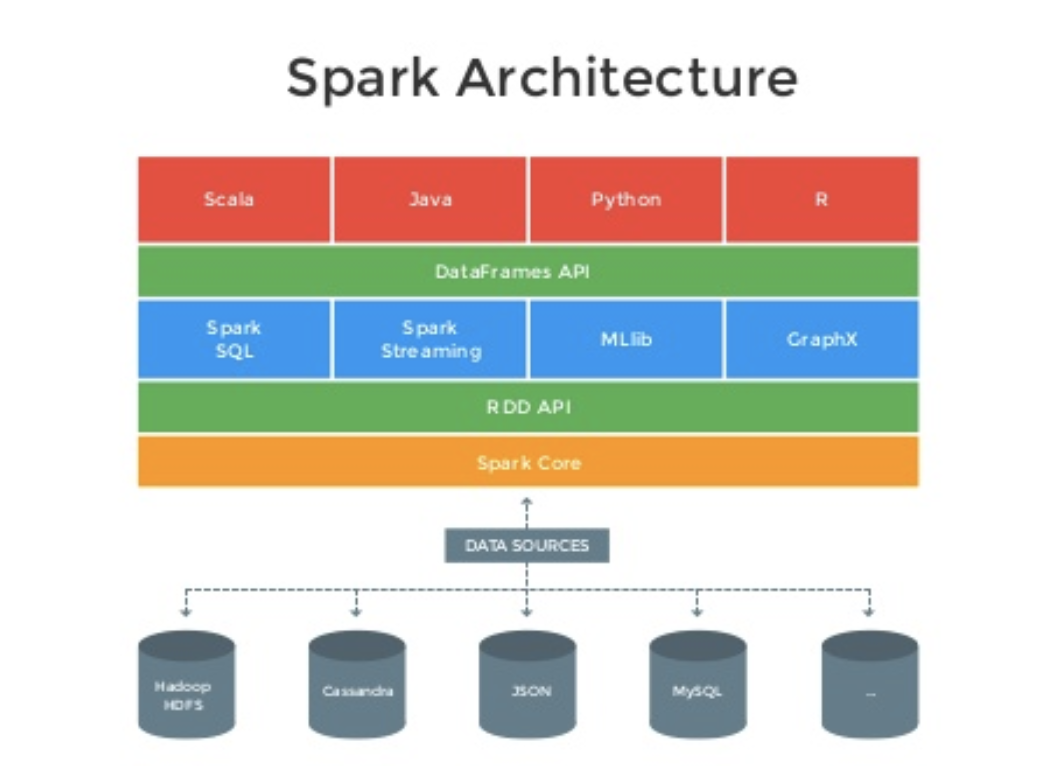
\includegraphics[width=\columnwidth]{images/Sparkarchic.png}
  \caption{Spark Architecture \cite{sparkarchitecture:fig}}
  \label{fig:sparkarchi}
\end{figure}

Spark's architectures given in the figure \ref{fig:sparkarchi} provide a glimpse of how different system in Spark is interfaced. The first level of interfacing to Spark is with high-level languages like Scala, Java, Python and R. Users implement their functionalities in these high -level languages. The primary executing components in Spark are Driver and Executor modules. The driver is the entry point for any implementation, the written programs will be executed in the main function of the Driver module, later converted to set of Directed Acyclic graph by the Spark APIs. DAGs are then executed in executors in the data nodes based on the data placement policy of the infrastructure. Four modules built on spark for serving the user's needs are SparkSQL, Spark Streaming, MLlib, and GraphX. Spark SQL and Machine Learning libraries(MLlib) are consumed in our implementation and the future improvement would be on Spark Streaming which is used for Streaming requirements. SparkSQL and MLlibs modules contain the implementation for DataFrames, SQL functionalities, and Machine learning libraries. The next level of the modules is data abstraction layer. Spark's basic data abstraction is Resilient Distributed Dataset (RDD), which is a fault tolerant partitioned data encapsulation datatype. The RDDs are lazily evaluated, hence a Directed Acyclic Graph is implemented to persist the state of the RDDs at each stage. With RDD, Spark can execute the transformation in parallel with fault tolerance. This implementation widely differentiates from conventional Python implementation which lacks this advanced logic.
Apache's Spark 2.2 is used to implement all the ETL functionality. Spark is installed is the local system along with Anacondas, so Spark libraries can be consumed inside Python shell. To consume and process Pyspark libraries, sparkcontext is created which initiates the driver program. The spark context is bootstrapped with SQL and Spark session libraries so that Spark RDD and Data frames could be accessed under a single window.

As the abstract describes the necessity of the features impacting Bitcoin's price, the best metric to identify the relation between Bitcoin's price and its features is by identifying the correlation matrix provided by Charles Spearman. Spearman's function describes the relationship between two variable using a monotonic function \cite{Spearman9:online}. Apart from identifying the correlation, these features can be modeled to predict the value of the dependent variable which is Bitcoin's value. The algorithm consumed for the predictions are Random forest and gradient boosted regression the Machine learning modules of Spark.

\section{Architecture}
The architecture flow consists of three levels of components, first one is the Data extraction, second is processing and the final is visualization. The Figure \ref{Architecture:project} describes how the implementation is fitted over Spark's architecture.
The logical implementation starts with extracting the data from the source and loading it over RDDs. With RDDs on the base, source data is validated for data miss and anomalies. With RDDs, all validation happens in parallel irrespective of any volume or variety of data. As RDDs are hash partitioned by default, it can consume any volume or type of data with consistent efficiency. Upon loading into RDDs, it is transformed to named columns as Dataframes which are indexed and more efficient in processing structured data. Pyspark dataframe is selected to increase the performance of the data processing even though Pyspark dataframe API is not equipped with rich functionalities similar to Pandas dataframe and Pyspark dataframe can execute the transformations in parallel whereas Pandas cannot. Machine learning algorithms are implemented over the Dataframes and generated model is executed and persisted as array objects for visualization.

\begin{figure}[!ht]
  \centering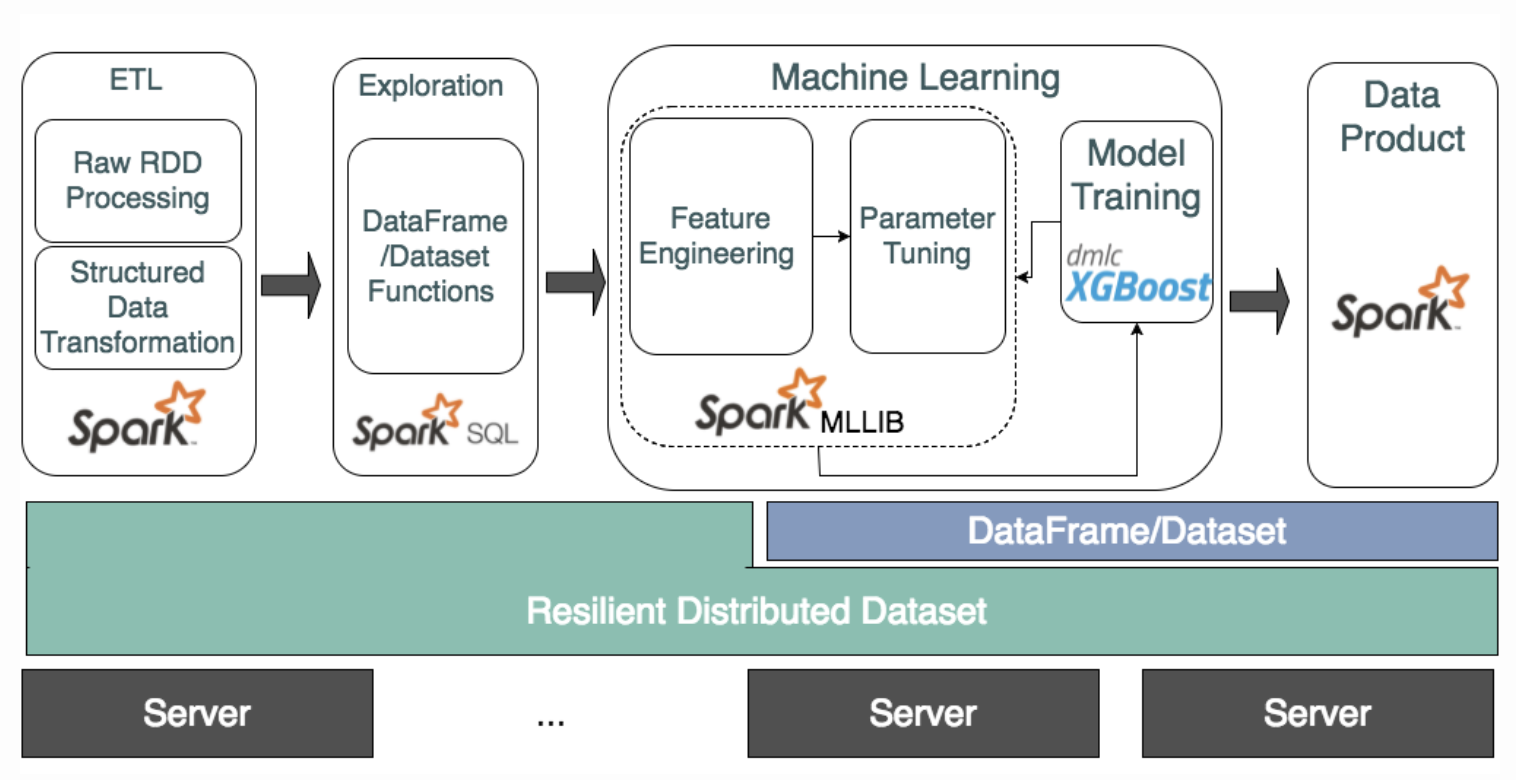
\includegraphics[width=\columnwidth]{images/Projectflow.png}
  \caption{Project Architecture on Spark \cite{project:fig}}
  \label{Architecture:project}
\end{figure}


\subsection{Technologies}

Technology stacks used in our implementation are, 
\begin{itemize}
\item Python 2.7 
\item Pyspark 2.2
\item Jupyter 5.0.0
\end{itemize}


\subsection{Data Extraction}
The data is sourced from Quandl.com, a public data service for various types of data, Bitcoin's mining data from 2015 till current date from Coinbase's mining pool. The data is in CSV format with Bitcoin's transaction details and its corresponding date associated with it.

The second set of data is from Etherscan, an open source portal for Ethereum transaction details, from which the transaction count and the price in US dollars are extracted.
The third dataset is about the people's trends on Bitcoin's popularity from Google, the granularity of this data is on weekly basis, hence it has to transformed statistically to fit into our model.

The first data set is programmatically downloaded with an API call with a private key authenticating it. {\em wget } is used in downloading the data within Shell script.
The later ones are downloaded manually from Google and Etherscan sites manually. The volume of the dataset is low, however, the volume increases as the consumption are initiated in real-time.

\begin{figure}[!ht]
  \centering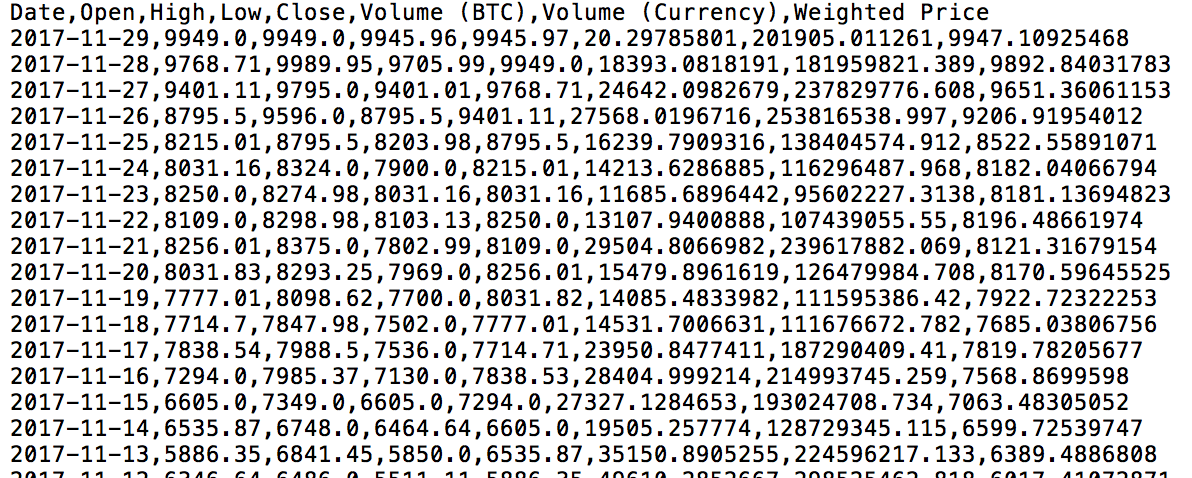
\includegraphics[width=\columnwidth]{images/Source1data.png}
  \caption{Bitcoin mining statistics data \cite{3:online}}
  \label{fig:sourcedata}
\end{figure}


Figure \ref{fig:sourcedata} describes the snapshot layout of one of the source data. It has 8 columns about the Bitcoin statistics segregated on per day basis. The first column is the date at which the other columns are recorded, the second is the opening price of the Bitcoin compared to USD on that day, likewise third, fourth and fifth columns pertains to high, low and closing rates of Bitcoin. The sixth column represents BTC's transaction count on that day and seventh is the volume in terms of USD value, at last is the weighted price 

\begin{figure}[!ht]
  \centering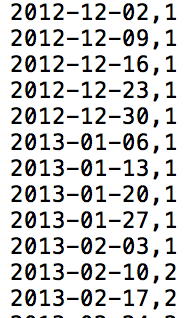
\includegraphics[width=0.18\columnwidth]{images/googledata.png}
  \caption{Google's trend data \cite{google:online}}
  \label{fig:googledata}
\end{figure}

\begin{figure}[!ht]
  \centering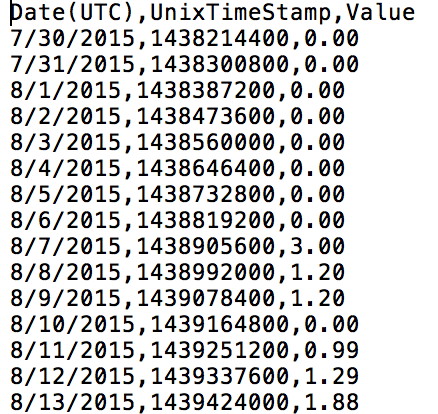
\includegraphics[width=0.4\columnwidth]{images/ethprice.png}
  \caption{Ethereum's pricing on daily basis \cite{Ethereum:online}}
  \label{fig:ethpri}
\end{figure}

\begin{figure}[!ht]
  \centering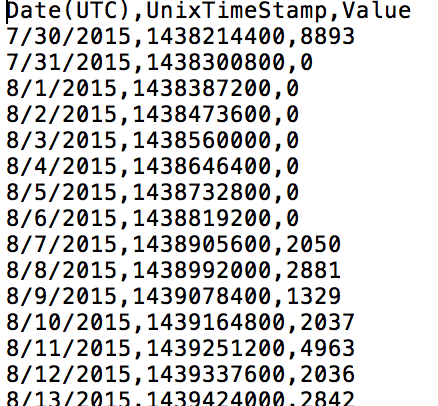
\includegraphics[width=0.4\columnwidth]{images/ethtran.png}
  \caption{Ethereum transactions on daily basis \cite{Ethereum:online}}
  \label{fig:ethtran}
\end{figure}

Figures \ref{fig:googledata}, \ref{fig:ethpri}, \ref{fig:ethtran} are the other features gathered from Google and Ethereum's mining pool. 

\subsection{Data Cleansing}
The data cleansed with multiple Python and feature cleansing libraries in Python and Pyspark. Major efforts of cleansing are needed to standardize the date columns from all the data sources. The date format was in the different format in different sources. To stitch back all the data points, Date Time libraries were used and joined with a single standard format. Another important activity in the cleansing is data miss. For some instance, the values are missing resulting in incorrect predictions and correlations. To resolve these missing values, Imputer \cite{imputer:online} functionality is used from feature library of Apache Spark. The imputer is an Imputation estimator for completing missing values, either using the mean or the median of the columns in which the missing values are located. The input to this function is dataframe columns and output are renamed dataframe columns. The processing happens in-memory with the spark.

\subsection{Data Visualization}
The visualization is provided in the form of static plots. Static plots are built-dimensional plots and scatter plots to represent correlation and projections.

\section{Spearman's correlation}
Spearman's correlation function is used to identify the correlation between Bitcoin's price and the features selected. In Spark, a separate function is defined to calculate Spearman's correlation. The input is in Pyspark RDD's and the output value is returned between -1 to +1. The positive ratio indicates the feature is directly proportional and the negative values indicate indirect proportionality.

Spearman's Correlation on the selected features are :

\begin{itemize}
\item BTC-volume    :0.348540857386 
\item High        :0.998581861669 
\item Low         :0.995190604708 
\item Open        :0.997943642437  
\item Google-trend:0.260343238604  
\item ETH price   :0.68683414787  
\item ETHTRAN     :0.720031468617
\item BTC-price-Label:1.0 
\end{itemize}

Per Spearman's correlation algorithm, highest correlations with Bitcoin's price are with trading data like High, low and Opening values of Bitcoin. Thee second highest correlation is with the Ethereum's transaction data. The least ones are Google's trend and Bitcoin's own transaction volumes.
These features are selected and used for the pattern analysis and prediction with regression algorithms. 


\begin{figure}[!ht]
  \centering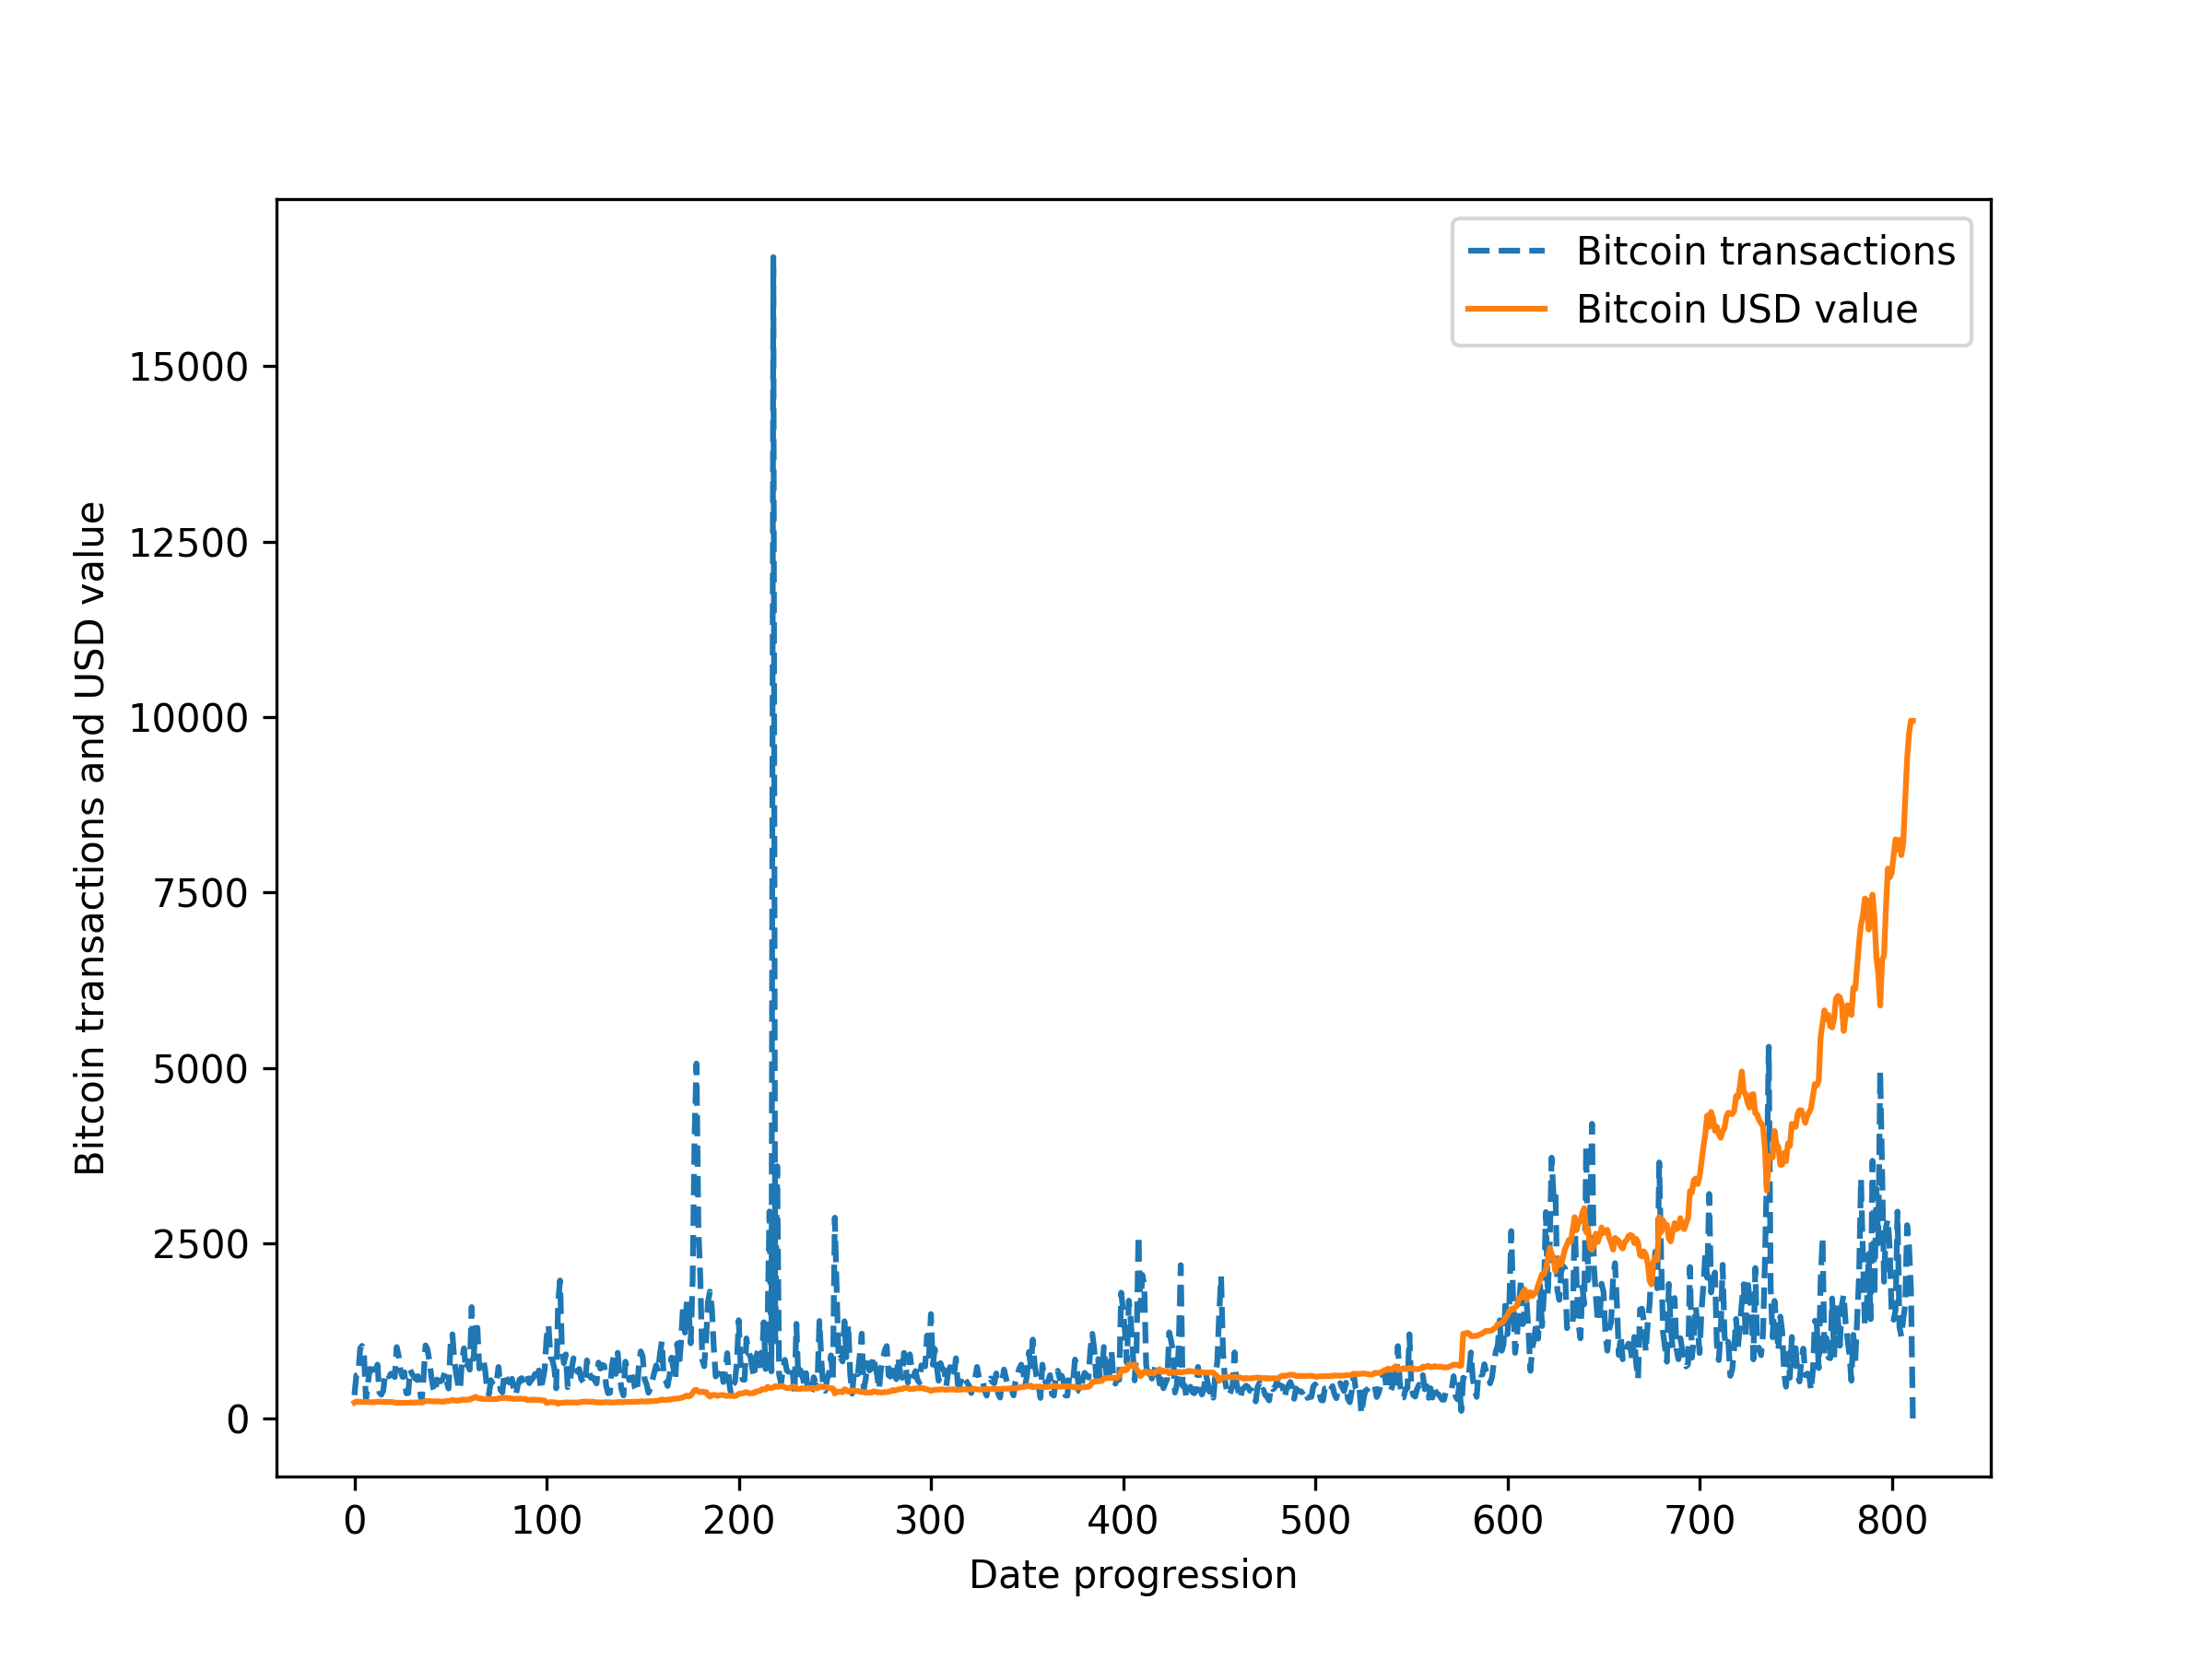
\includegraphics[width=\columnwidth]{images/BTC-prcvsBTC-trans.png}
  \caption{Bitcoin Transaction and USD value }
  \label{1}
\end{figure}

The Figure\ref{1} describes the growth pattern between Bitcoin transaction count and its value. The y-axis is the count of Bitcoin's transactions and the x-axis is the date progression, it means day 0 on considered as the July 30,2015 and the next day is considered as 1. What is inferred from the correlation is that the volatility of the transactions increased as the price increases and in other perspective the transaction counts are moderately consistent even though the value is increasing which means some other feature impacting the price more than the number of transactions. 

\begin{figure}[!ht]
  \centering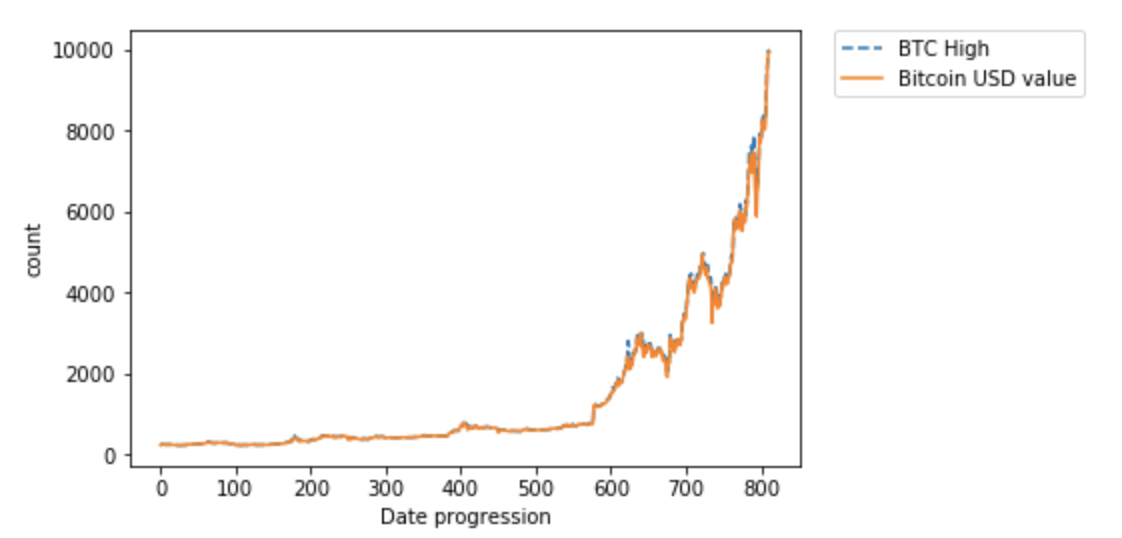
\includegraphics[width=\columnwidth]{images/High.png}
  \caption{Bitcoin Highest exchange value and Closing value}
  \label{2}
\end{figure}

\begin{figure}[!ht]
  \centering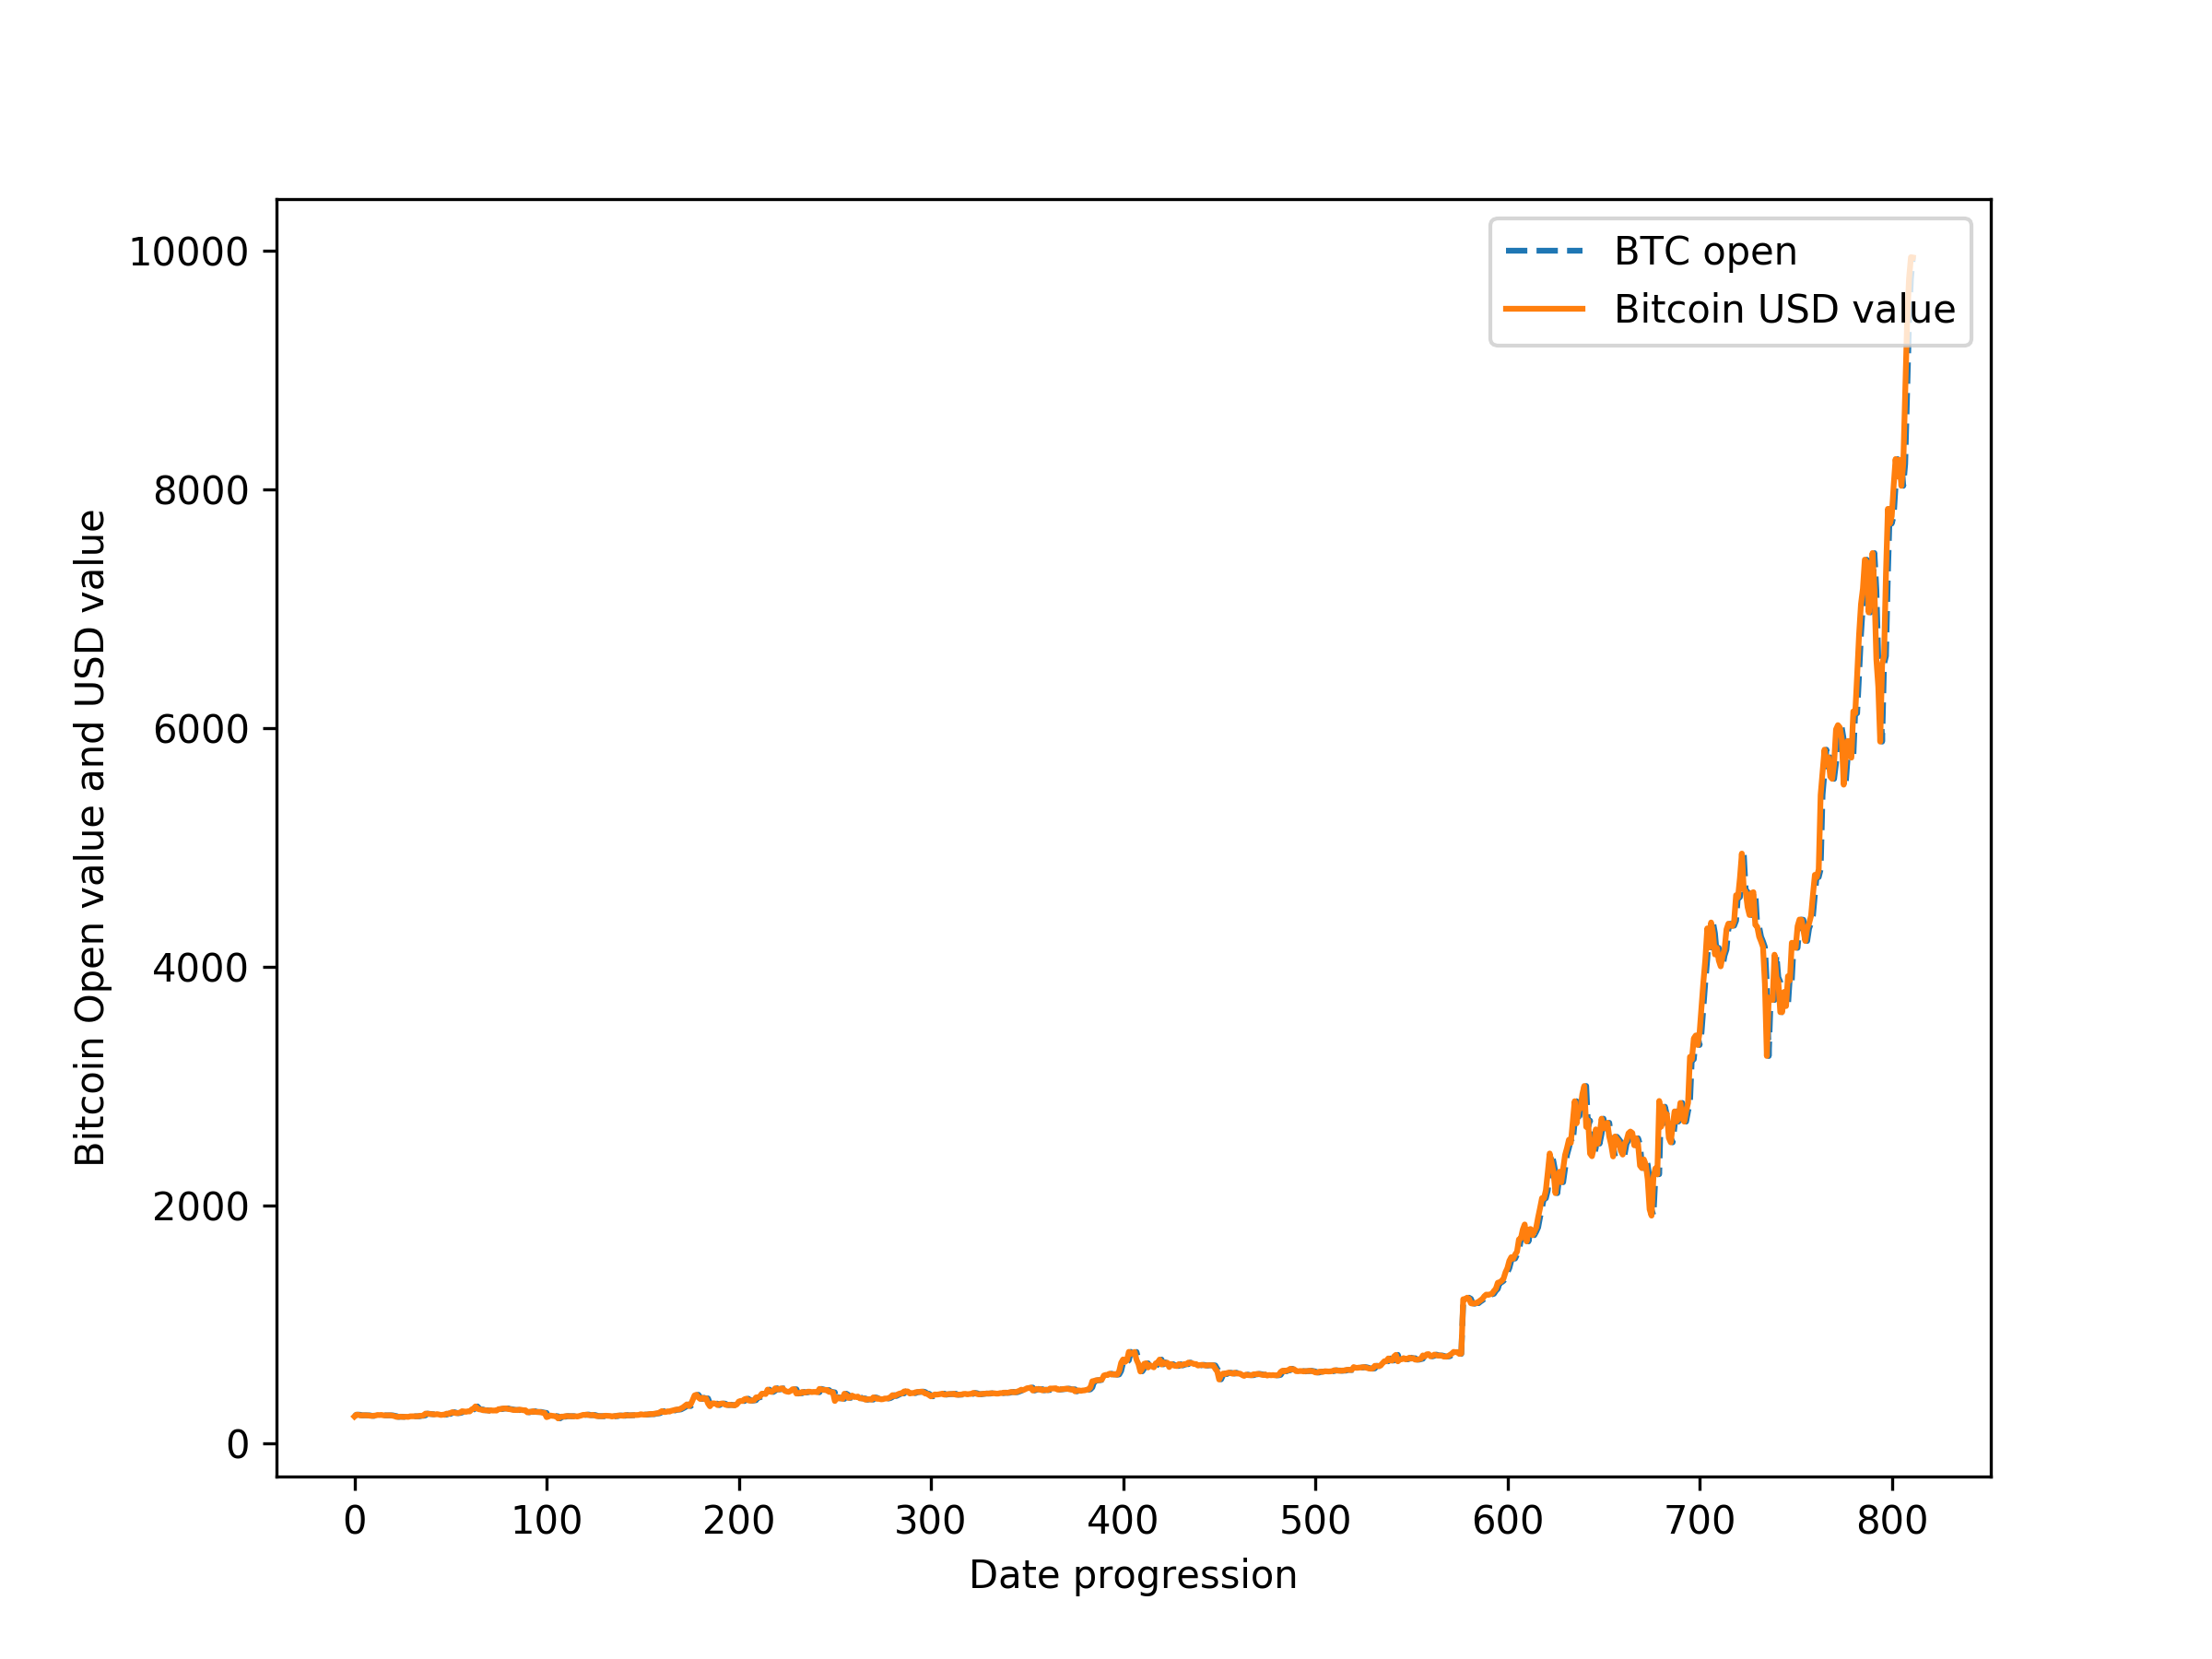
\includegraphics[width=\columnwidth]{images/Open.png}
  \caption{Bitcoin Lowest exchange value and Closing value }
  \label{3}
\end{figure}

\begin{figure}[!ht]
  \centering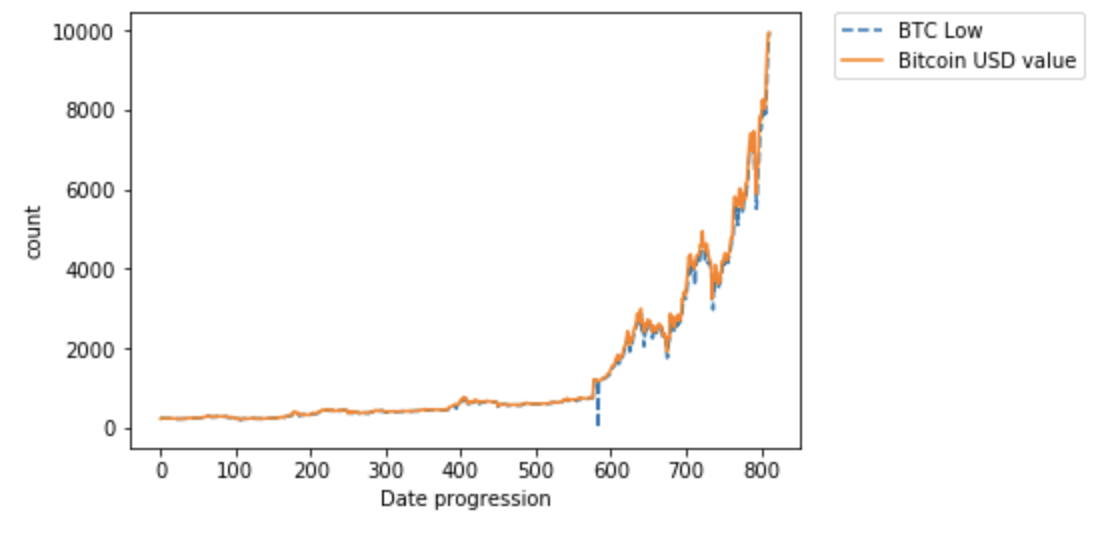
\includegraphics[width=\columnwidth]{images/low.png}
  \caption{Bitcoin Opening exchange value and Closing value}
  \label{4}
\end{figure}

The Figures \ref{2},\ref{3} and \ref{4} describes the growth pattern between open, low and high prices of Bitcoin on the recorded date.
The x-axis is date progression and the y-axis is the value of Bitcoin's price and Bitcoin's highest, opening and lowest price on that day. This is obvious that these prices are highly correlated with the price change.

\begin{figure}[!ht]
  \centering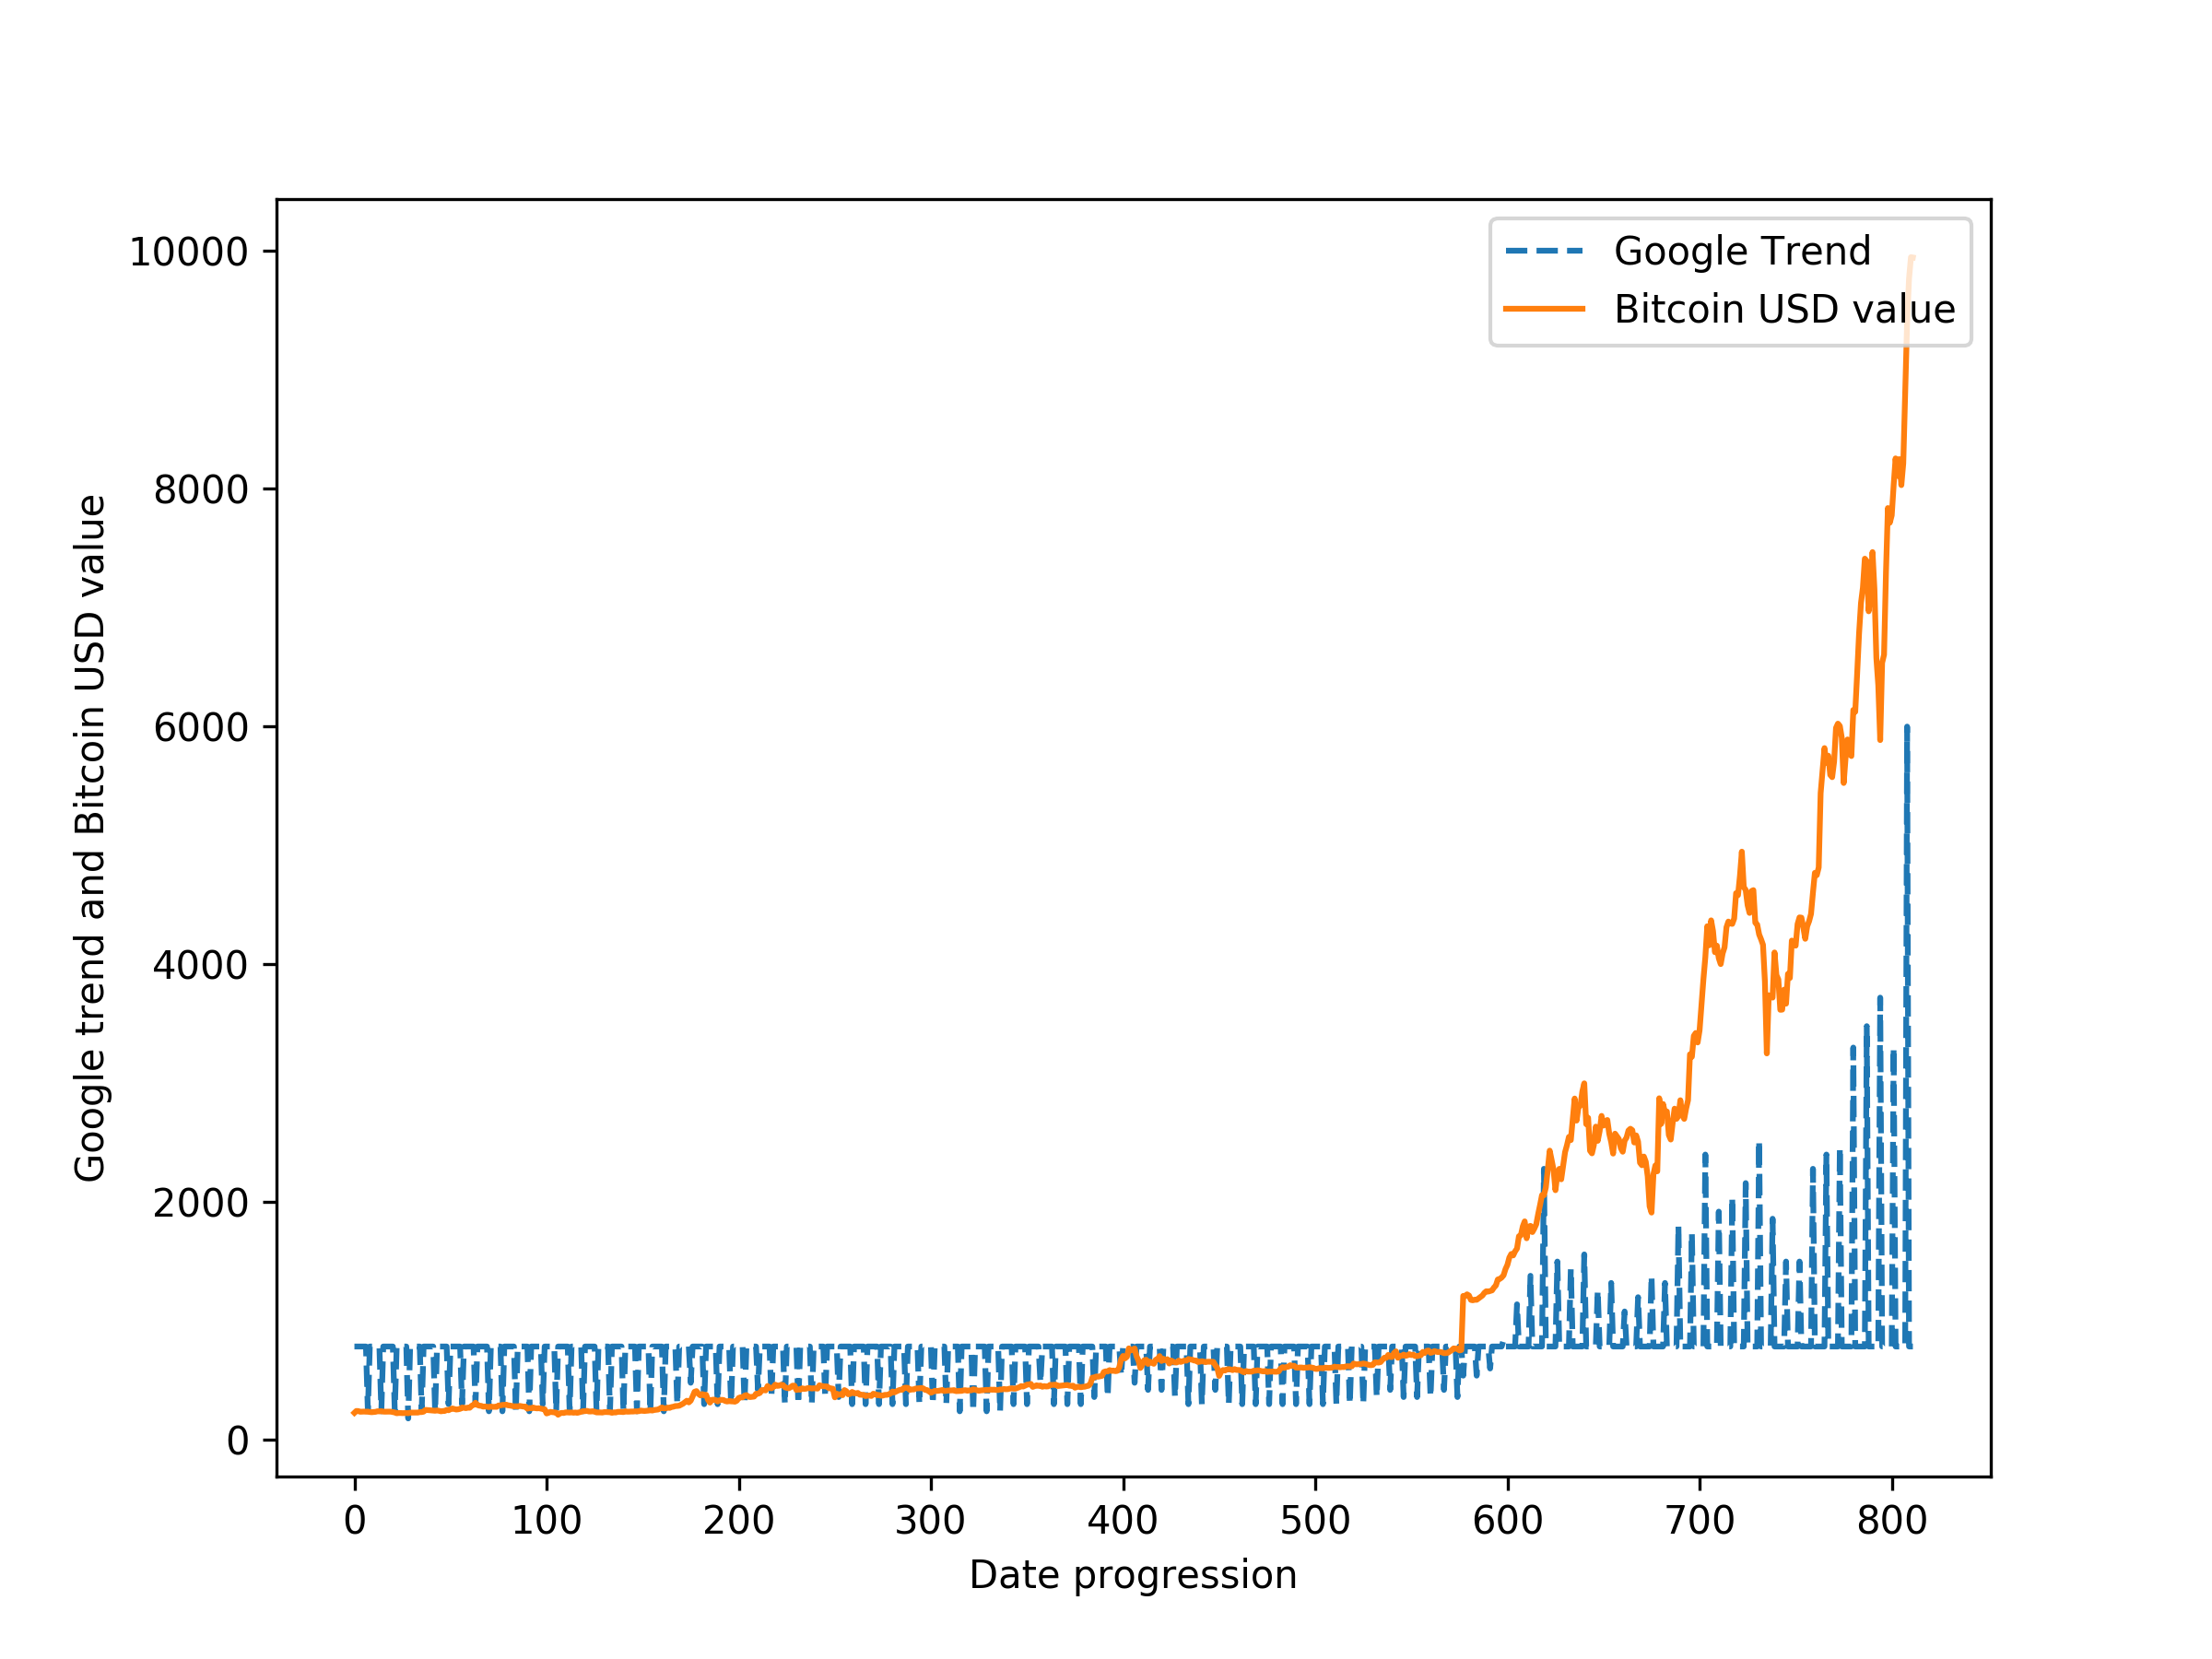
\includegraphics[width=\columnwidth]{images/googletrend.png}
  \caption{Bitcoin USD value and Google search trend}
  \label{5}
\end{figure}

The figure \ref{5} describes the pattern between the Google search trend and the hike in Bitcoin's price, the x-axis in the Date progression and the y-axis defines the counts of the features. 

\begin{figure}[!ht]
  \centering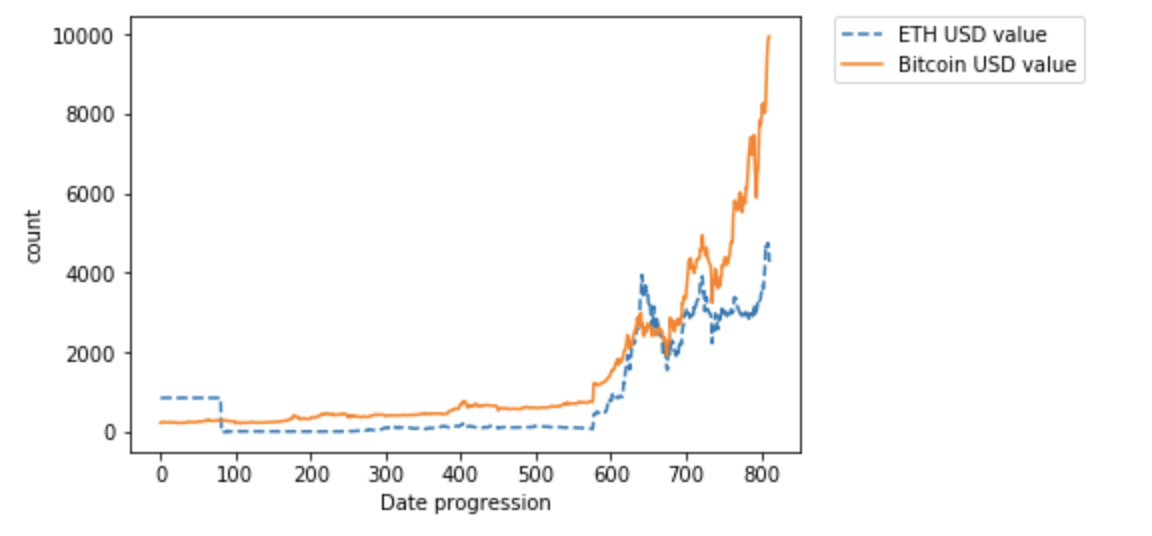
\includegraphics[width=\columnwidth]{images/ethvalue.png}
  \caption{Ethereum price and Bitcoin price}
  \label{6}
\end{figure}

\begin{figure}[!ht]
  \centering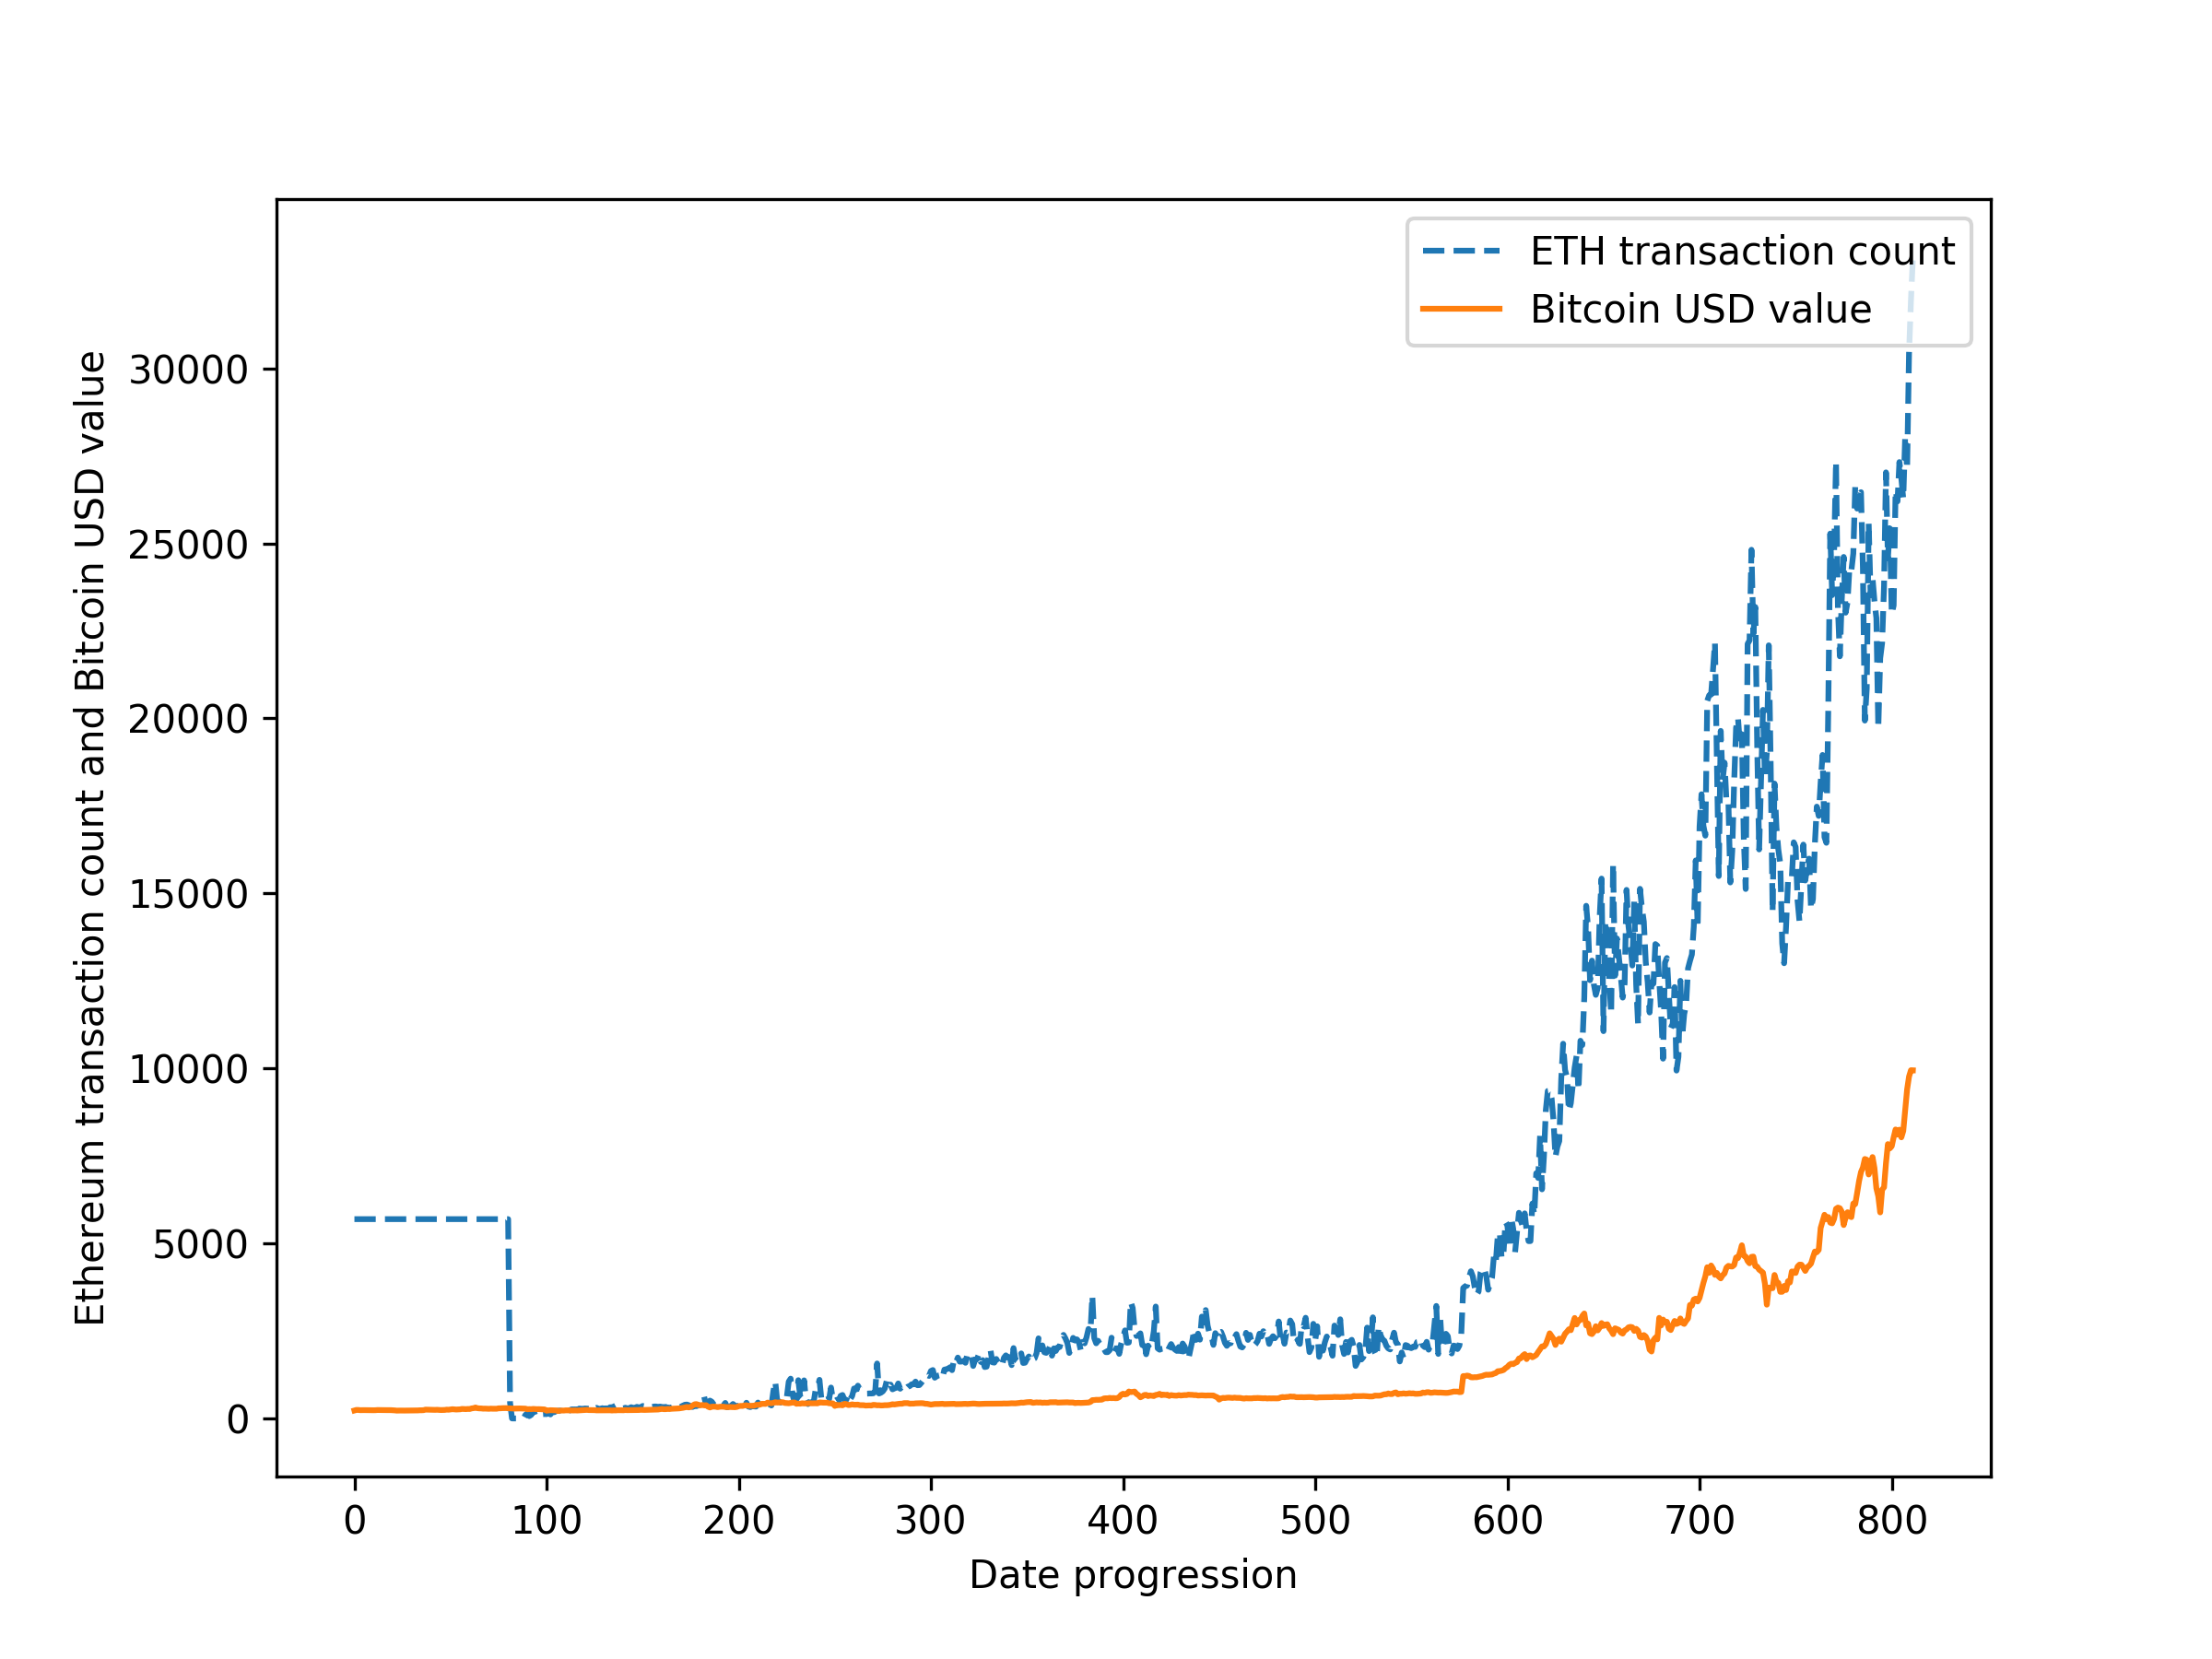
\includegraphics[width=\columnwidth]{images/ethtrancount.png}
  \caption{Ethereum Transaction volume and Bitcoin transaction volume}
  \label{7}
\end{figure}

Figure \ref{6} and \ref{7} describes the growth trend of Ethereum's price and its transaction volumes with Bitcoin's price in which the transaction pattern of Ethereum is more similar to Bitcoin's pattern. 

As far as processing is concerned, all the RDDs are cached before feeding into Spearman's correlation function, the reason being, when the RDDs are transformed multiple times, it has to calculate data lineage every time it is computed and lineage is the basic quality of resilience in Apache Spark. If the RDDs are cached and persisted in-memory, the iteration and other transformations happen in memory avoiding costly I/O operations, this feature cannot be easily implemented when executed in conventional python libraries.


\section{Decision Tree Regression}
With the availability of features, we can take the processing to the next level of predicting Bitcoin's price. Here, supervised learning model is used to predict the price of Bitcoin.

\begin{figure}[!ht]
  \centering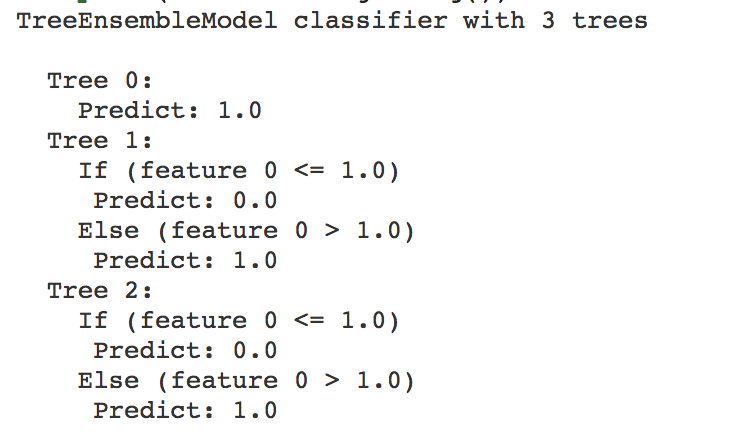
\includegraphics[width=0.75\columnwidth]{images/Decisiontree.png}
  \caption{Sample Decision tree}
  \label{fig:8decisiongree}
\end{figure}
 

Figure \ref{fig:8decisiongree} give some basic idea of how decisions are made with the supervised decision tree based model.

Ensemble method models are derived from another base model. The base model used here is Decision trees and ensemble models are Random forest and Gradient Boosted tree(GBT) Algorithms.

Though the base model for both the algorithms is same, both are different in terms of training the dataset. GBT can train only one tree at a time whereas Random forest can train multiple trees resulting in reduced overfitting caused by GBTs.

''Random forests or random decision forests operate by constructing a multitude of decision trees at training time and outputting the class that is the mode of mean prediction (regression) of the individual trees and GBTs iteratively train decision trees in order to minimize a loss function. Like decision trees, GBTs handle categorical features, extend to the multiclass classification setting, do not require feature scaling, and are able to capture non-linearities and feature interactions''\cite{Ensemble4:online}.

All the execution is implemented in Apache Spark, hence all the transformation and processing happens in-memory, even if the data volume is high, the processing will spawn across the clusters and will be processed with consistent redundancy.

The model is implemented by first splitting the data into two sets of different volume, i.e test data and training data. The training data will be used by the model to derive the logic and the built logic will be tested with the test data for accuracy. Here, 70:30 ratio is selected for training and test data respectively. And by altering this ratio we can adjust the performance of the model. Upon completion of the modeling, the accuracy of the models is calculated based on Metrics library in Spark. The metrics identified for the accuracy calculations are mean Squared Error, Root Mean Squared Error, r-square and mean Absolute error. Mean Squared error can be defined as an estimator to measures the average of the squares of the errors or deviations \cite{MSE}. ''R-squared is a statistical measure of how close the data are to the fitted regression line. It is also known as the coefficient of determination, or the coefficient of multiple determination for multiple regression'' \cite{rsq:online}.



\subsection{Random Forest}
As we are predicting Bitcoin's USD value per day, Bitcoin's price in considered as a label and all other columns are marked as features, and only the features having a decent level of correlation is marked as Features. These features are loaded into the model with Labelled Points as a Spark dataframe.

Random forest requires parameters to tune the model for the highest accuracy. 

The parameters used in the functions are \cite{api:docs} :
\begin{itemize}
\item Training dataset: RDDs as LabeledPoint
\item NumTrees: Number of trees in the random forest
\item FeatureSubsetStrategy: Number of features to consider for splits at each node
\item Impurity: Criterion used for information gain calculation 
\item MaxDepth: Maximum depth of tree
\item MaxBins: Maximum number of bins used for splitting features
\item Seed: Random seed for bootstrapping and choosing feature subsets
\end{itemize}

The first parameter is the training dataset, the training datasets are constructed as LabelledPoint RDDs, the LabelledPoint RDD is a local vector associated with a label, it acts as a optimized data structure for datasets with association. The next one is the number of trees allowed to construct in the algorithm, as the decision tree is based on deriving mean of multiple decision trees, in general, more trees gives better results. However, the improvement decreases as the number of trees increase more than the threshold of the given dataset. Hence, number of trees selected is {\em 10}, which gives us better efficiency. The FeatureSubsetStrategy defines how the features are sampled at each split in a tree, we have selected {\em auto}, so the algorithm will take care of the split. The Impurity parameter is the criteria followed for Information gain calculation, {\em variance} is the default considered by Spark. The next parameter is MaxDepth, which defines the limit of the depth of the tree, beyond which decision tree will not be extended, the maximum depth allowed in Spark is {\em 30}. The next one is MaxBins, which describes the number of bins used for splitting which we have defaulted and the last one is Seed parameter, which induces randomness while multiple trees are created which is defaulted as well.

With all parameters were carefully selected and the model is tuned to give the highest accuracy, Avg.closeness index of the algorithm is closer to 0.95. After deriving the model, the closeness/correctness of the predicted results was also analyzed and it is described in the plot \ref{scpl:ran}.

\subsection{Gradient Boosted Tree}
In the Gradient Boosted algorithm, the training and test data are used in similar to the Random Forest algorithm. The implementation is less complex compared with Random forest. As GBT trains the model based on iterative execution of sequence of decision trees. Upon execution of three iterations, it is clearly evident with the closeness index that the data is little bit over-fitted with the closeness index of 0.96, slightly greater than Random forest.

The parameters used in the functions are \cite{api:docs} : 
\begin{itemize}
\item Training dataset: RDDs as LabeledPoint
\item CategoricalFeaturesInfo: A Map of categorical features
\item Loss Function: Loss function used for minimization during gradient boosting
\item NumIterations: Number of iterations of boosting
\item LearningRate: Learning rate for shrinking the contribution of each estimator
\item MaxDepth: Maximum depth of tree 
\item MaxBins: Maximum number of bins used for splitting features.
\end{itemize}

Similar to Random Forest, the first parameter is LabelledPoint RDD,
the second one the map of categorical features. Most important parameters used in GBT's functionality are Loss function, NumInterations and Learning rate. Loss function selected is {\em leastSquaresError}. Number iteration is the number of times the tree is iterated to derive the result, the default value of {\em 100} is selected. The learning rate is optional which is defaulted to {\em 0.1} in Spark.

By altering these parameters, the performance and the decision of the model can be optimized. The alteration includes thorough analysis of the data consists of data gap analysis and feature transformation.
By selecting the default parameters, the output decision tree tend to perform better in the selected scenario.

\section{Results}

From the observation of scatter plots of regression model Random forest \ref{scpl:ran} and GBT \ref{scpl:gbt}, it is evident that GBT's single tree iterative model has predicted the values with over-fitting. Some predicted values are consistent with some particular time scope and changes happening in steps. The prediction distribution looks like a single line and not widespread. Whereas, in the Random forest, the predicted values are widespread and closely aligned.

\begin{figure}[!ht]
  \centering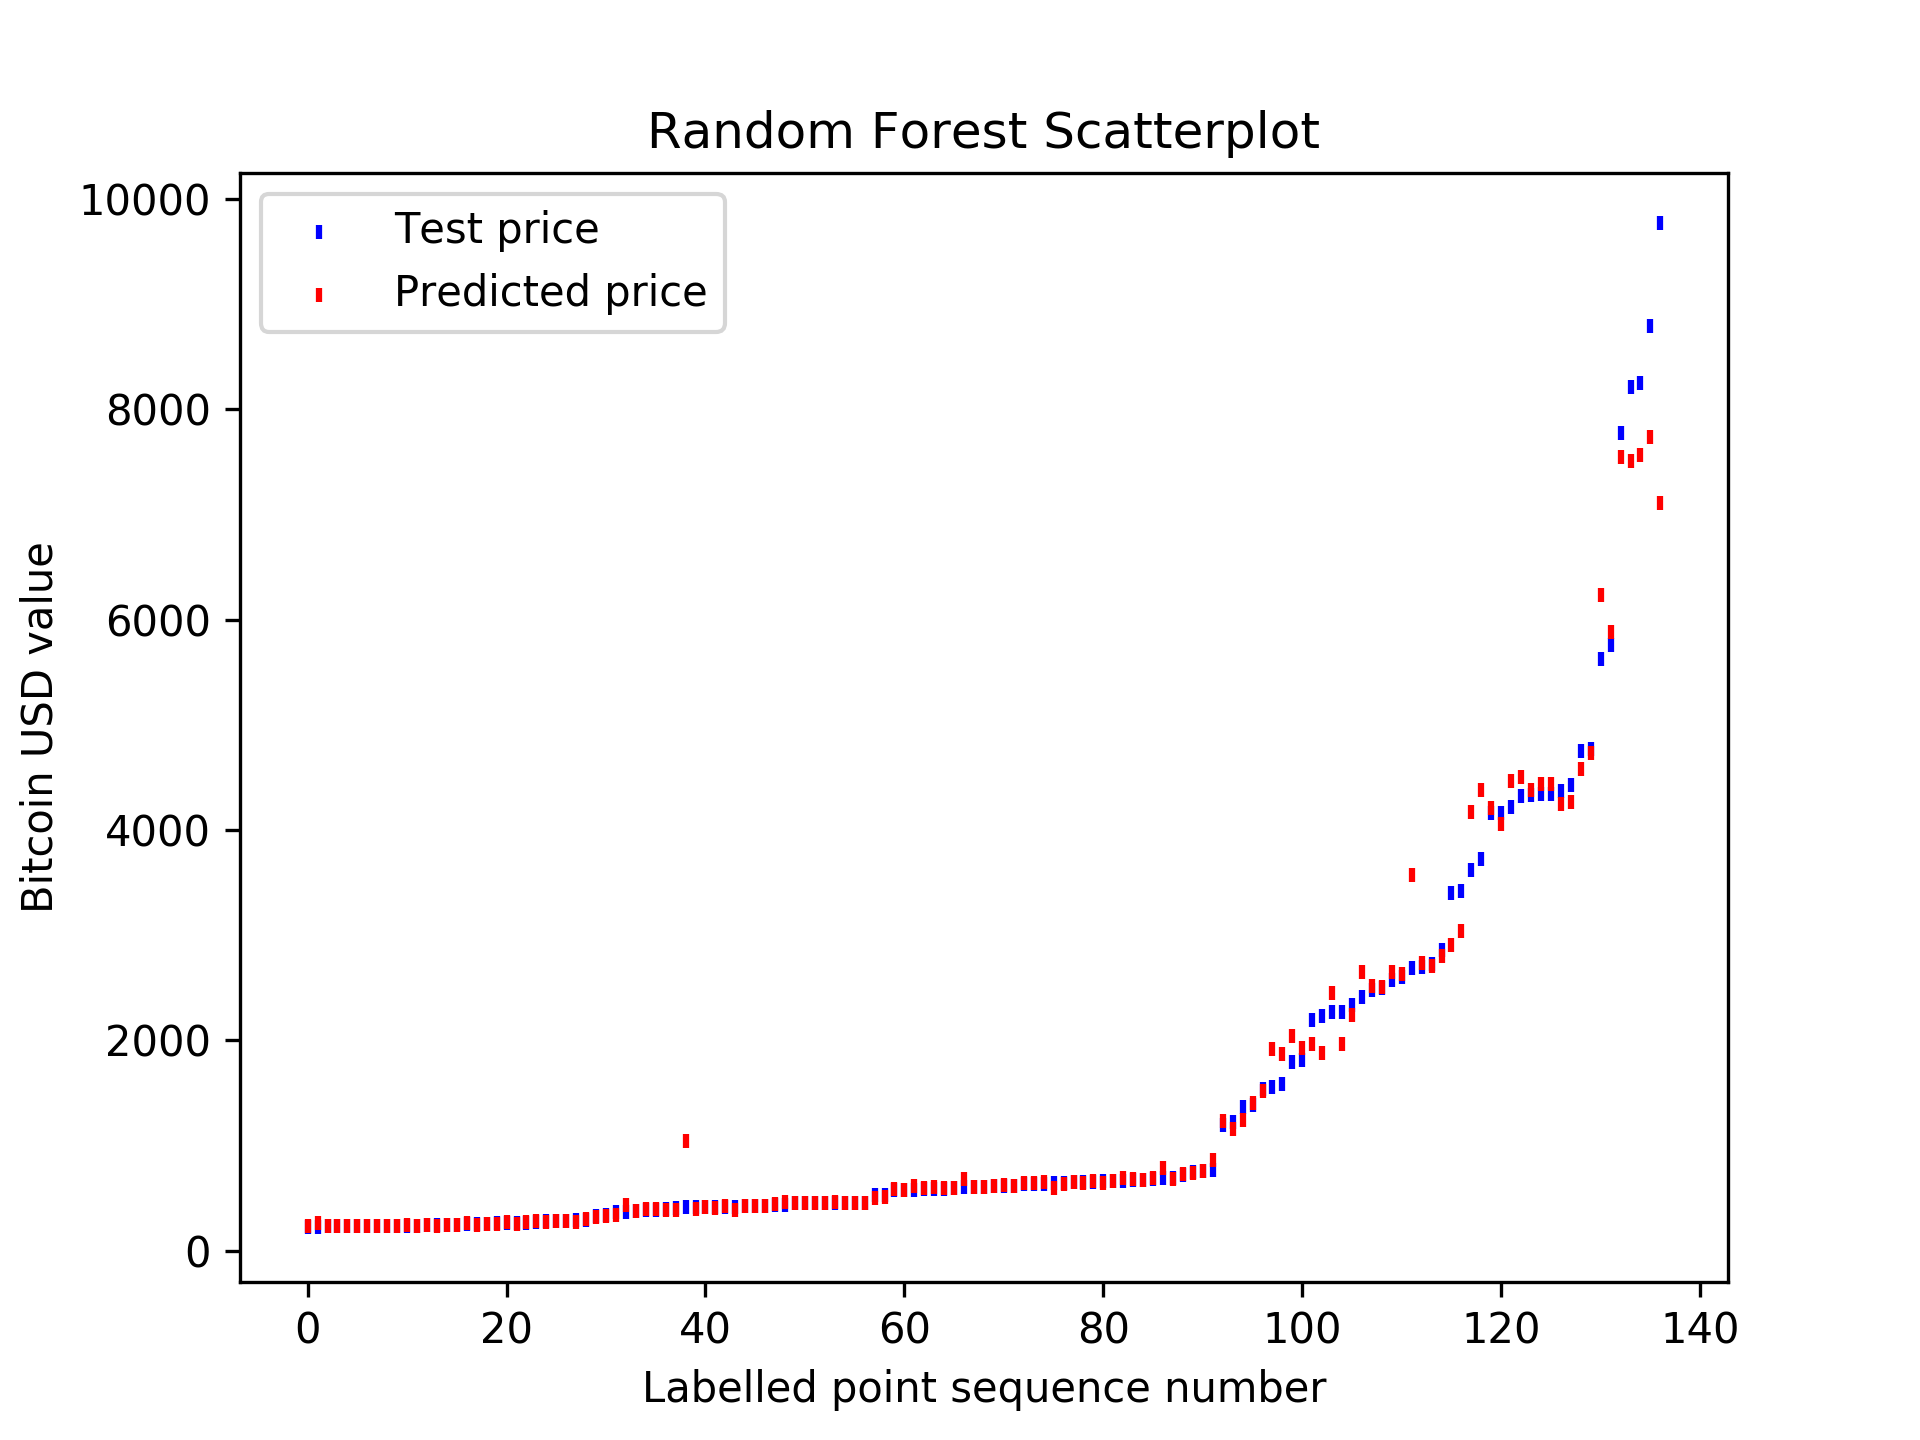
\includegraphics[width=\columnwidth]{images/RandomForestscatterplot.png}
  \caption{Randomforest Scatterplot}
  \label{scpl:ran}
\end{figure}

\begin{figure}[!ht]
  \centering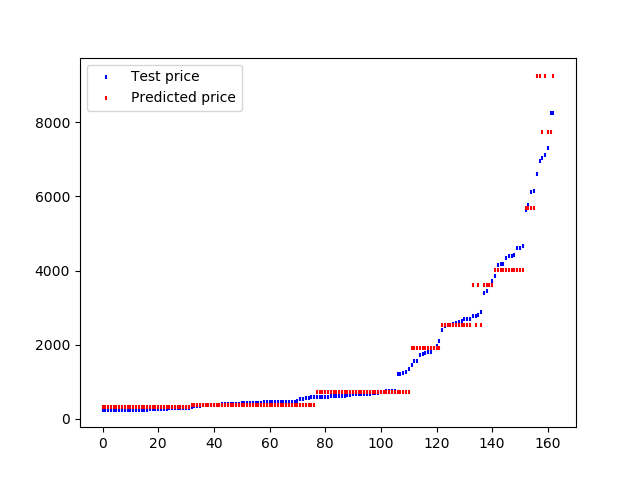
\includegraphics[width=\columnwidth]{images/GBTscatterplot.png}
  \caption{Gradient Boosted Tree Scatterplot}
  \label{scpl:gbt}
\end{figure}

We have came up with a metric called {\em Closeness indicator}, which tells us mean ratio of test and predicted label. If it is less than 100, then the predicted value is less than the actual and if it is more than 100, then the predicted value is more than the actual value.
For both algorithms, the closeness index is near 100\%, hence both predictions achieved optimal results. Other important metric includes r-square values which above 95\% in both the cases, hence our model fits with the expectation and the parameter selected for the algorithm holds good. 



\section{Challenges faced}
Most of the challenges are with the data and casting to the required data types as the correlation and regression functions need data either in float or double data types. The other challenge faced is the data source availability, though the Bitcoin network is open to the public, gathering all the statistics data from all the mining pool available in BTC infrastructure is tedious. And, in the Bitcoin network, we do not know which user performs the transaction, we have no open option to classify the user and identify the feature inducing that transaction. Due to the void of these inducing factors, we may need to assume few features and start the analysis with the correlation. And handling all these constraints along with Big data specifics in mind adds up to the challenge, thanks to Apache Spark which handles the data lineage and persistence through RDDs. 

\section{Project structure}
Three folders are created, the first one is for scripts which retain the actual code to be executed and two Korn shell scripts to install dependencies and to download the required source files. The second one is the data folder which retains the data required for the model and correlation algorithm. The extract folder is to persist the plot figures extracted out of the python script. The versioning and multiuser synchronization is supported by Git. 

\section{Improvement Opportunities}
There are a lot of improvement opportunities to be implemented in the project. One of them includes fetching the data in near real-time directly from the Mining-pool instead of a third party data service, the second one would be increasing the granularity of data which would increase the performance and the Spark would make more sense with that level of granularity and volume. The other improvement opportunities include gathering more features like illegal market transaction data, mining exchange data, wallet exchange data, world's inconsistency data which will increase correlation factors and result in the accurate prediction of models. Other visualization opportunity includes real-time presentation capabilities with Big Data at the back end. Matplot API has minimal options for real-time reporting which can be upgraded.
Other important improvement opportunity includes implementing the prediction logic with Neural network based models like Long Short-Term Memory(LSTM) as decision tree based models sometimes fail to adapt to the changes based on their past experience. These LSTM based model keep the memory of the previous experience and improve the learning upon training.

\section{Conclusion}
After the analysis of the Bitcoin data, the Bitcoin transaction count does not impact the Bitcoin's value which proves that the users are not using the Bitcoin for any day to day transactions instead they are exchanging it with US Dollars and saving as an asset like Gold. By retaining it, the demand for the Bitcoin coin increases. As the new-coins can only be generated through mining and the growth is controlled, coins in circulation keep reducing, increasing its cost further. It clearly proves that Bitcoin bought are saved in the wallets are not used in the regular transaction much. Most of the Bitcoin's are retained to earn the profit over its demand and its price variation with US Dollars. Other important inference is that the exchange rate of Ethereum is changing along with Bitcoin's, the only possibility of close correlation is the exchange of both the currencies. By logically linking the findings, people are using Bitcoin as an asset and using other cryptocurrencies as the transaction medium exchanged from Bitcoin's market instead of directly from the US Dollar market.

With all prowess of Big Data and its technologies, Blockchain technologies are not only evolving, it also equips humans with the opportunity to make the world more transparent, ethical and a viable place to live. As the technology has evolved so far, it is expected to understand its growth story in terms of its microscopic level to push it to the next level of improvement. Such microscopic level of qualities was missed in legacy methods and Big Data comes to the rescue in identifying those qualities and nurture them.


\begin{acks}
  The authors would like to thank Dr. Gregor von Laszewski for his support and suggestions to write this paper.
\end{acks}

\bibliographystyle{ACM-Reference-Format}
\bibliography{report} 



\end{document}
